A system is judged by the quality of the services it offers and its ability to function reliably. Even though the reliability of operating systems has been studied for several decades, it remains a major concern today. The characteristics of the operating systems which make them unstable are size and complexity. 
\\[3mm]
Coverity analysis of the Linux kernel shows that the Linux kernel 2.4.1 source code has 1000 bugs, and Linux kernel 2.6.9 source code has 950 bugs. The study also shows that 53\% of the bugs are present in the device drivers~\cite{coveritykernel}. 
\\[3mm]
In Linux, memory protection prevents a user process from accessing memory that has not been allocated to it. Memory protection is a way to control memory access rights. It prevents a bug within a user process from affecting other processes, or the operating system~\cite{Denning:1970:VM:356571.356573, Galvin}. Linux kernel modules do not have the same level of isolation the user level applications have. Unlike user applications, the Linux kernel has thousands of procedures linked together. In the Linux kernel, any portion of the kernel can access and potentially overwrite any kernel data structure used by an unrelated component. Such a non-existent isolation between kernel and device driver causes a bug in device drivers to corrupt the memory of the other kernel components. This memory corruption sometime leads to system crash. The underlying cause of the unreliability in the operating system is the lack of isolation between device driver and Linux kernel.

\pagebreak

\section {Problem Statement}
\label{sec:problem}
In the past, solutions to increase the reliability of a system, based on virtualization has been proposed by LeVasseur et. al.~\cite{LeVasseur04UnmodifiedDriverReuse}, Xen isolated driver domain system~\cite{Fraser04safehardware}. These solutions improve the reliability of the system by executing device drivers in an isolated environment from the kernel. The use of virtual machines has a well-deserved reputation for extremely good fault isolation. In a virtualized environment, none of the virtual machines are aware of the other virtual machines, and malfunctioning of one virtual machine cannot spread to the others. Xen hypervisor also provides a similar platform to isolate device driver from the monolithic kernel. The platform is called driver domain~\cite{driverdomain}.
\\[3mm]
Despite the advances in virtualization technology, the overhead of I/O virtualization significantly affects the performance of applications~\cite{Barham:2003:XAV:945445.945462, Sugerman:2001:VID:647055.715774, Menon:2006:ONV:1267359.1267361}. In this thesis, we propose and evaluate an optimization for improving the performance of the driver domain under the Xen. 
\pagebreak
  
\section {Proposed Solution} 
Virtualization based solutions explained in the section~\ref{sec:problem} exploit the memory protection capability between virtual machines. In a virtualized environment, all virtual machines run as separate user processes in different address spaces. The Xen isolated driver domain system runs user applications and a kernel in a guest domain, and runs a device driver in a separate domain. As a result, a device driver is isolated from the Linux kernel running in a guest domain, making it impossible for the device driver to corrupt any kernel data structure in the virtual machine running user applications. In this thesis, we re-implement the Xen isolated driver domain system and call it as Isolated Device Driver (IDDR). Our solution to improve the performance of the Xen isolated driver domain system is implemented over the IDDR base code.
\\[3mm]
\begin{figure}[!ht]
\centering
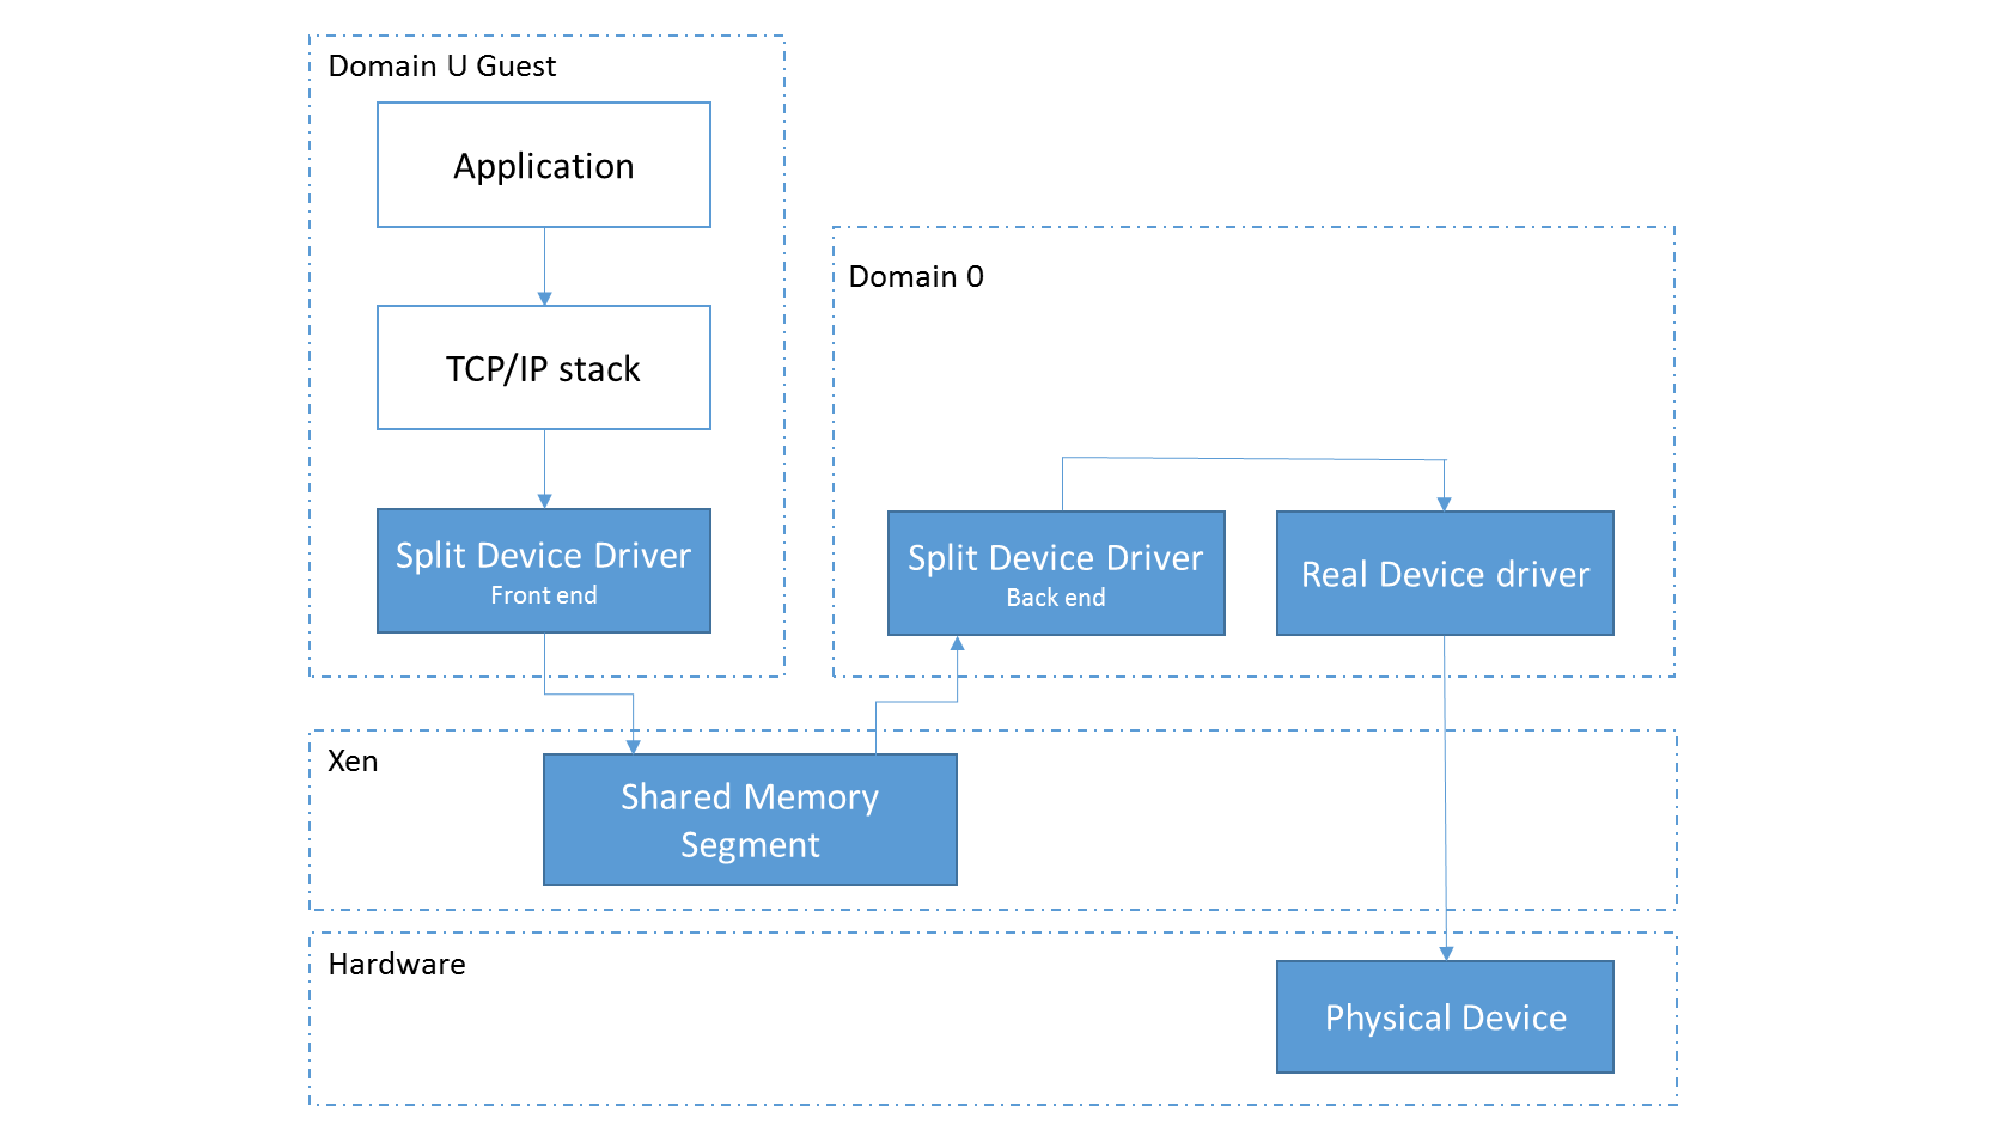
\includegraphics[scale=.50]{xen-split-tcp.pdf}
\caption{Split device driver model}
\label{fig:xen-split}
\end{figure}
Xen VMM does not include device drivers for all the devices, adding support for all the devices would be a duplication of effort. Instead, Xen delegates hardware support to a guests. The guest typically runs in priviledged domain, although it is possible to delegate hardware to guests in other domains. Model in which hardware support is delegated to a guest is called split device driver model~\cite{Chisnall:2007:DGX:1407351}. Xen uses the same split device driver model in isolated driver domain as shown in the figure~\ref{fig:xen-split}.
\\[3mm]
Xen has a front end driver in the guest operating system and a back end driver in the driver domain. The front end and the back end driver transfer data between domains over a channel that is provided by the Xen virtual machine monitor. Within the driver domain, back end driver is used to de-multiplex incoming data to the device and to multiplex outgoing data between the device and the guest domain~\cite{driverdomain}.
\\[3mm]
The Xen isolated driver domain system follows an interrupt based approach in the communication channel~\cite{Barham:2003:XAV:945445.945462}. In this communication model, front end and back end notifies each other the receipt of a service request and corresponding responses by sending an interrupt. This interrupt based model requires context switches~\cite{Barham:2003:XAV:945445.945462}. In a multitasking system, context switch refers to the switching of the CPU from one process or thread to another. Context switch makes multitasking possible. At the same time, context switch causes unavoidable system overhead~\cite{Li:2007:QCC:1281700.1281702, Mogul:1991:ECS:106973.106982}. Hence the overhead is caused by the communication channel in the Xen driver domain. 
\\[3mm]
In order to improve the performance of the communication channel, we propose a solution in which a thread in the back end driver spins for the service request, and the front end driver spins for the availability of the corresponding responses. As the front end driver spins for the responses, and spinning does not involve any context switch, our solution performs better than the Xen isolated driver domain system.
\\[3mm]
The performance of the system is evaluated over block devices such as ramdisk device, loop device, and SATA disk. The raw block device is formatted with a file system and the IDDR system is evaluated by measuring the performance of the system with fileIO/SysBench benchmark. The integrity of the system is checked by executing raw read/write, read/write ahead, read/write superblock, sync and flush tests on the block device. The evaluation of our solution shows that the performance of the system can be improved by avoiding the context switches in the communication channel. 
 \pagebreak

\section{Core Contributions}
The core contributions of this project are listed below. 
\begin{enumerate}
\item Re-implementation of the Xen driver domain - Isolated Device Driver (IDDR).
\item Improvement in the performance of IDDR by implementing thread based communication channel instead of interrupt based communication channel. 
\item Our performance comparison of the thread based IDDR and interrupt based IDDR.
\end{enumerate}

\pagebreak
\section {Organization}
This section gives the organization and roadmap of the thesis.
\begin{enumerate}
\item Chapter 2 gives the background on Processes, threads, Memory protection, Virtualization, Hypervisor and inter-domain communication.
\item Chapter 3 gives the introduction to design of the system to isolate device driver. 
\item Chapter 4 discusses the detailed design and implementation to isolate device driver. 
\item Chapter 5 evaluates the performance of Independent device driver with different designs.
\item Chapter 6 reviews the related work in the area of kernel fault tolerance.
\item Chapter 7 concludes the report and lists down the topics where this work can be extended.
\end{enumerate}

\ifbool{toShowBibliography}{\bibliography{references}}{}